\documentclass{article}
\usepackage{tikz, comment}
\usepackage{pifont}
\usepackage{fontspec}
\usetikzlibrary{arrows, decorations.markings, decorations.pathreplacing}
\begin{comment}
:Title: Not defined yet
:Tags: absolute value rules;properties of equality, equation rules;equation of a line;trichotomy;equivalence properties of equality
:Prob: 0.5082;0.4473;0.4347;0.4263;0.4231
:Author: Prof.Hu Ji-shan, HKUST
:Slug: No name yet

Description Here.........
\end{comment}
\begin{document}\centering

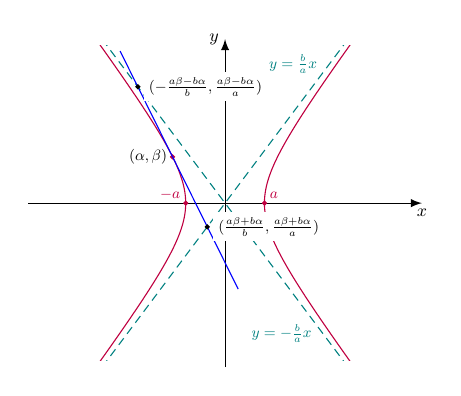
\begin{tikzpicture}[>=latex,xscale=.5/6, yscale=.5/6][font=\sf\small]

%\draw[xstep=1cm,ystep=1cm,color=gray!80] (0, -1) grid (8, 8);

\draw[->] ({-30}, 0) -- ({30}, 0)node[below, scale=0.7] {$x$};
\draw[->] (0, {-25}) -- (0, {25})node[left, scale=0.7] {$y$};

\draw[purple, fill, xscale=6, yscale=6] ({6/6}, {0/6}) circle(0.05)node[right, xshift=0, yshift=3, scale=0.6] {$a$};
\draw[purple, fill, xscale=6, yscale=6] ({-6/6}, {0/6}) circle(0.05)node[left, xshift=0, yshift=3, scale=0.6] {$-a$};

\node[teal, left, xshift=2, yshift=6, scale=0.6] at ({14}, {4/3*(14)}) {$y = \frac{b}{a}x$};
\node[teal, left, xshift=0, yshift=-3, scale=0.6] at ({14}, {-4/3*(14)}) {$y = -\frac{b}{a}x$};

\foreach \x in {}
\draw (\x,2pt*1) -- (\x,-2pt*1)
node[anchor=north] {\tiny$\x$}
;
\foreach \x in {}
\draw (\x,2pt*1.5) -- (\x,-2pt*1.5)
node[anchor=south] {\tiny$\x$}
;
\foreach \y in {}
\draw (-2pt*1,\y) -- (2pt*1,\y)
node[anchor=east] {\tiny $\y$}
;

\clip[] (-30, -24) rectangle (30, 24);

\draw[purple, samples=100, smooth, domain=-2:2, variable=\t]
plot ({sqrt(36)*(exp(\t)+exp(-\t))/2}, {sqrt(64)*(exp(\t)-exp(-\t))/2});

\draw[purple, samples=100, smooth, domain=-2:2, variable=\t]
plot ({-sqrt(36)*(exp(\t)+exp(-\t))/2}, {sqrt(64)*(exp(\t)-exp(-\t))/2});

\draw[densely dashed, teal, samples=100, smooth, domain=-20:20, variable=\x]
plot ({\x}, {4/3*(\x)});

\draw[densely dashed, teal, samples=100, smooth, domain=-20:20, variable=\x]
plot ({\x}, {-4/3*(\x)});

\draw[purple, fill, xscale=6, yscale=6] ({-8/6}, {8*sqrt((8/6)^2-1)/6}) circle(0.05)node[left, black, scale=0.6] {$(\alpha, \beta)$};

\draw[blue, samples=100, smooth, domain=-16:2, variable=\x]
plot ({\x}, {8*sqrt((8/6)^2-1)+8^2*(-8)/(6^2*8*sqrt((8/6)^2-1))*(\x-(-8))});

\draw[fill, xscale=6, yscale=6] ({(-6*8*sqrt((8/6)^2-1)+8*(-8))/8/6}, {(6*8*sqrt((8/6)^2-1)-8*(-8))/6/6}) circle(0.05)node[right, black, fill=white, xshift=2, scale=0.6] {$(-\frac{a\beta-b\alpha}{b}, \frac{a\beta-b\alpha}{a})$};

\draw[fill, xscale=6, yscale=6] ({(6*8*sqrt((8/6)^2-1)+8*(-8))/8/6}, {(6*8*sqrt((8/6)^2-1)+8*(-8))/6/6}) circle(0.05)node[right, fill=white, xshift=2, scale=0.6] {$(\frac{a\beta+b\alpha}{b}, \frac{a\beta+b\alpha}{a})$};

%\node[scale=0.7] at ({-0.2*2.5*2}, {-0.2*2.5*2}) {\scriptsize$0$};

\end{tikzpicture}
\end{document}